\section{Wherein shade is thrown at terminal emulators}
\label{sec:termshade}
\epigraph{And as he spoke, El-ahrairah's tail grew shining white and flashed like a star;
and his back legs grew long and powerful and he thumped the hillside until the
very beetles fell off the the grass stems. He came out of the hole and tore across
the hill faster than any creature in the world.}{Richard Adams, \textit{Watership Down}}
The \texttt{notcurses-demo} program detailed in Chapter~\ref{sec:ncdemo} serves
as an excellent testbed for benchmarking certain properties of various
terminals in various configurations. The \texttt{-c} argument ought always be
provided when benchmarking, so that the PRNG is seeded with the same
value\footnote{This only serves to eliminate variance among equal PRNG
implementations.}. The \texttt{-J} argument is also useful, to generate JSON-formatted
output suitable for machine processing. Finally, \texttt{-d} can be supplied
to reduce the amount of artificial delay: the default is \texttt{-d1} for 1.0x
the standard delay. \texttt{-d0} eliminates all artificial delay.

This binary is composed of over a dozen
different independent demos, which can be freely scheduled on the command line.
Different demos have different usefulness for benchmarking. Fixed-time, fixed-framecount
demos will generally only show differences in the amount of time spent
rendering. Fixed-framecount demos show difference in total time. Fixed-time demos
might show differences in framecount and time spent rendering. A greater
number of frames for the same demo is indicative of an advantage, as is completing
any particular demo in less time. The most generally useful stat to compare
across runs is average time per render and maximum time to render.

\begin{table}[!htbp]
  \centering
  \begin{tabular}{ |c|c|c| }
    \hline
    Demo & Type & Exercises \\
    \hline
    \hline
    Intro & Fixed-time & Fades, EGC draws \\
    \hline
    X-Ray & Fixed-time+frame & Plane movement (x), video \\
    \hline
    Eagle & Time-to-completion & Large renders, multiple sprites \\
    \hline
    Trans & Fixed-time & Plane movement (xy) \\
    \hline
    \rowcolor{blue!25}
    \textbf{Highcon} & Time-to-completion & Intense RGB, intense redraw \\
    \hline
    Box & Time-to-completion & Intense redraw \\
    \hline
    Chunli & Fixed-time+frame & Large sprite \\
    \hline
    \rowcolor{blue!25}
    \textbf{Grid} & Time-to-completion & Intense RGB, RGB variance \\
    \hline
    Reel & Fixed-time & Plane movement (y) \\
    \hline
    Whiteout & Fixed-time & Intense font rendering \\
    \hline
    Uniblock & Fixed-time & Intense font rendering \\
    \hline
    View & Fixed-time+frame & Video \\
    \hline
    Luigi & Time-to-completion & Sprites, background \\
    \hline
    \rowcolor{blue!25}
    \textbf{Fallin} & Time-to-completion & Many planes, plane movement (y) \\
    \hline
    Sliders & Time-to-completion & Many planes \\
    \hline
    Jungle & Fixed-time & Palette cycling \\
    \hline
    Outro & Fixed-time & Fades, video \\
    \hline
  \end{tabular}
\caption[Benchmarking properties of various demos.]{Benchmarking properties of
  various demos. I consider the colored demos particularly informative.}
\label{table:benchmarks}
\end{table}

Prior work benchmarking terminal emulators largely focused on ``scroll speed'',
a fairly useless and easily misleading statistic\cite{lookatterms}, and input
latency\cite{typingpleasure}.

All of the following graphs have a logarithmic y-axis. At an 80x52 geometry,
the number of bytes output by different demos spans three orders of magnitude,
and the time (when all artificial delays are removed) by four orders of
magnitude\footnote{With artificial delays, it's more like a single order of
magnitude.}. The font family used is always Hack\cite{hacktypeface} at 10 points,
except for \texttt{xterm}, which became effectively unusable with this TrueType
font. I instead allowed \texttt{xterm} to use its default font and size, leading
to a much smaller total window size at the 80x52 cell geometry. Nonetheless,
\texttt{xterm} still reliably delivered the poorest performance\footnote{\textbf{FIXME FIXME FIXME investigate this}}.

All terminals were their Debian Unstable or Arch-packaged variants at the time
of testing, save \texttt{alacritty}, which was not yet present in Debian. Full
details are provided in Table~\ref{table:benchterms}.

\begin{table}
  \centering
  \begin{tabular}{|l|l|l|p{.4\textwidth}|}
    \hline
    Emulator & Version & \texttt{TERM} & Comments \\
    \hline
    \hline
    xfce4-terminal & 0.8.9.1 & vte-256color & \texttt{xfce4-terminal} is based on GNOME's VTE\cite{gnomevte}, as are a great many other distro-rebranded terminals. \\
    \hline
    xterm & Patch \#353 & xterm-256color & See note above regarding regression to bitmapped fonts, yuck. \\
    \hline
    kitty & 0.15.0 & kitty-direct & OpenGL-based \\
    \hline
    alacritty & 0.4.1-dev (4d3f6de) & alacritty & OpenGL-based \\
    \hline
    konsole & 19.08.1 & konsole-direct & KDE's terminal \\
    \hline
  \end{tabular}
\caption{Terminal software used for benchmarking.}
\label{table:benchterms}
\end{table}

\begin{figure}[!htb]
\centering
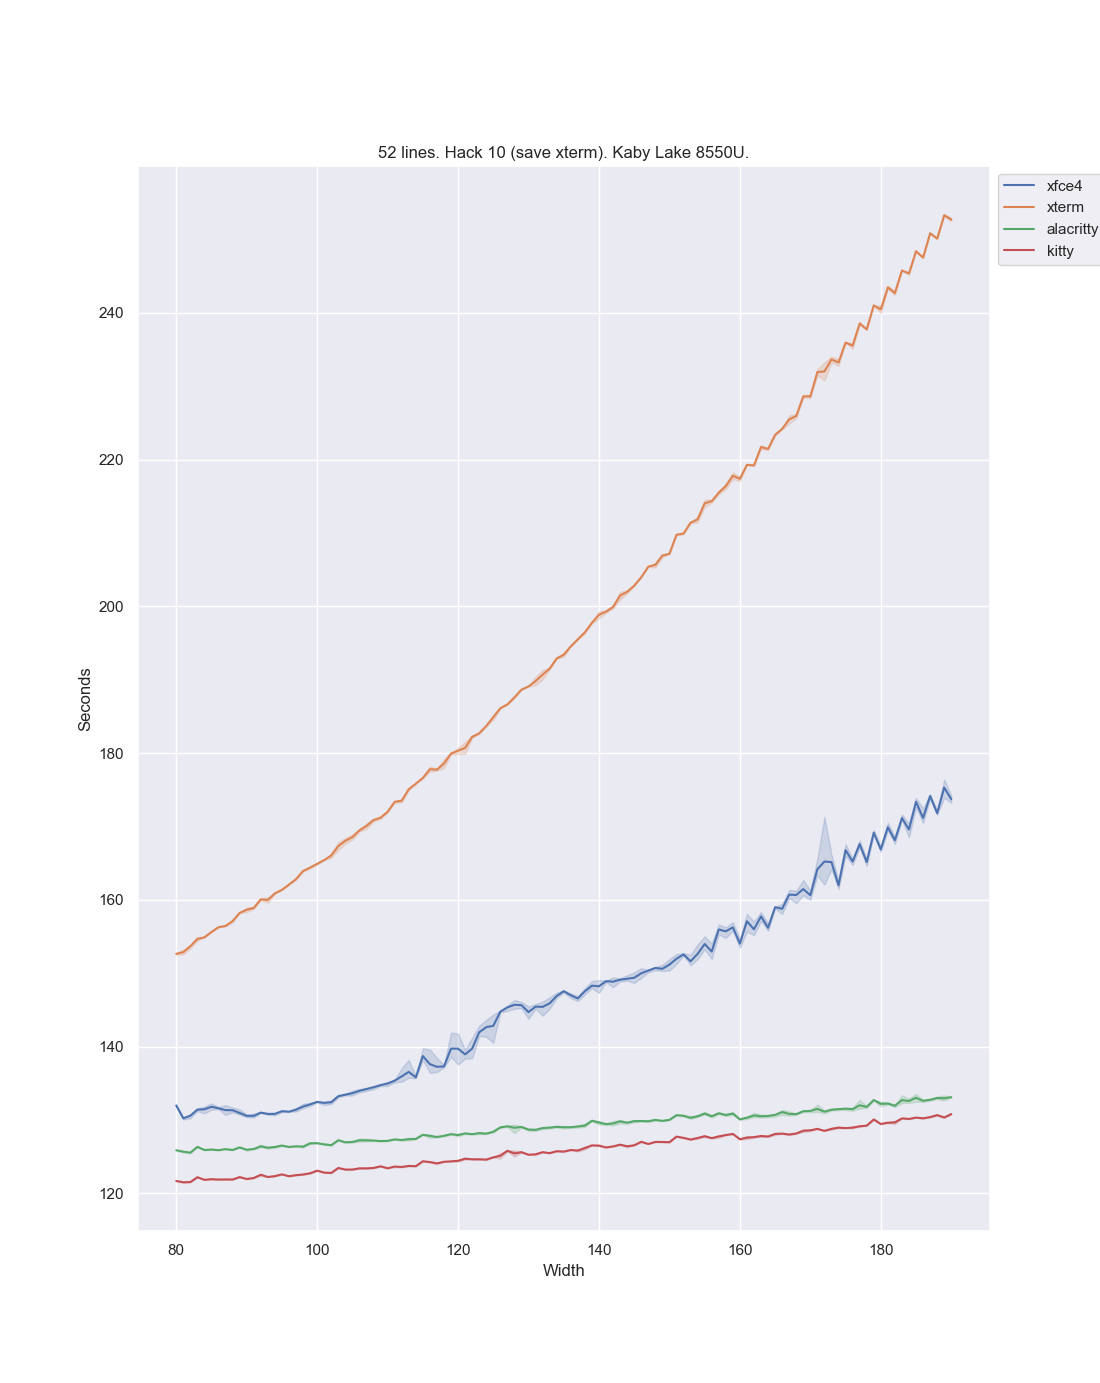
\includegraphics[width=1\textwidth]{media/termsdemo.png}
\caption[Intel i7-8550U benchmarks, varying widths.]{\texttt{notcurses-demo} runtime against terminal width (logarithmic y). Linux 5.5.2 + i915, Arch Xorg 1.20.7, no false delay. 3 runs each, at each width.
At this scale (about 100s), timings are very repeatable from run to run.}
\label{fig:intel-full}
\end{figure}

\begin{figure}[!htb]
\centering
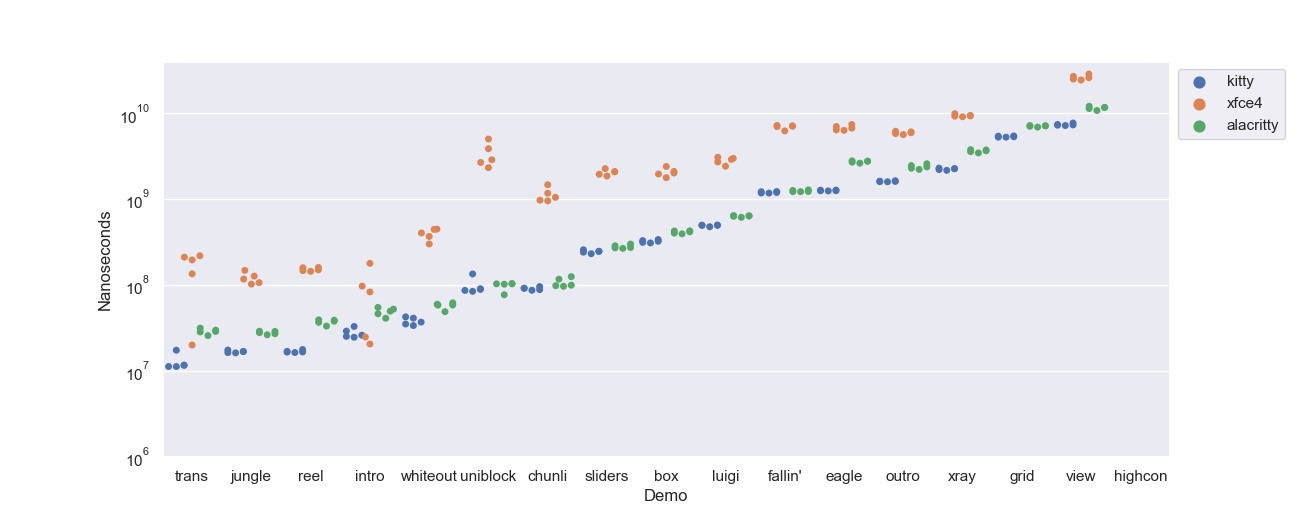
\includegraphics[width=1\textwidth]{media/d0-large-nvidia.png}
\caption[382x74 NVIDIA GTX 1080 benchmarks.]{Runtimes on a 382x74 geometry (logarithmic y) atop Linux 5.5.9 + NVIDIA GTX1080 440.64, Debian Xorg 1.20.7, no false delay. 5 runs each. VTE appears to scale much more poorly than the GL-based Kitty and Alacritty.}
\label{fig:nvidia-full}
\end{figure}

\begin{figure}[!htb]
\centering
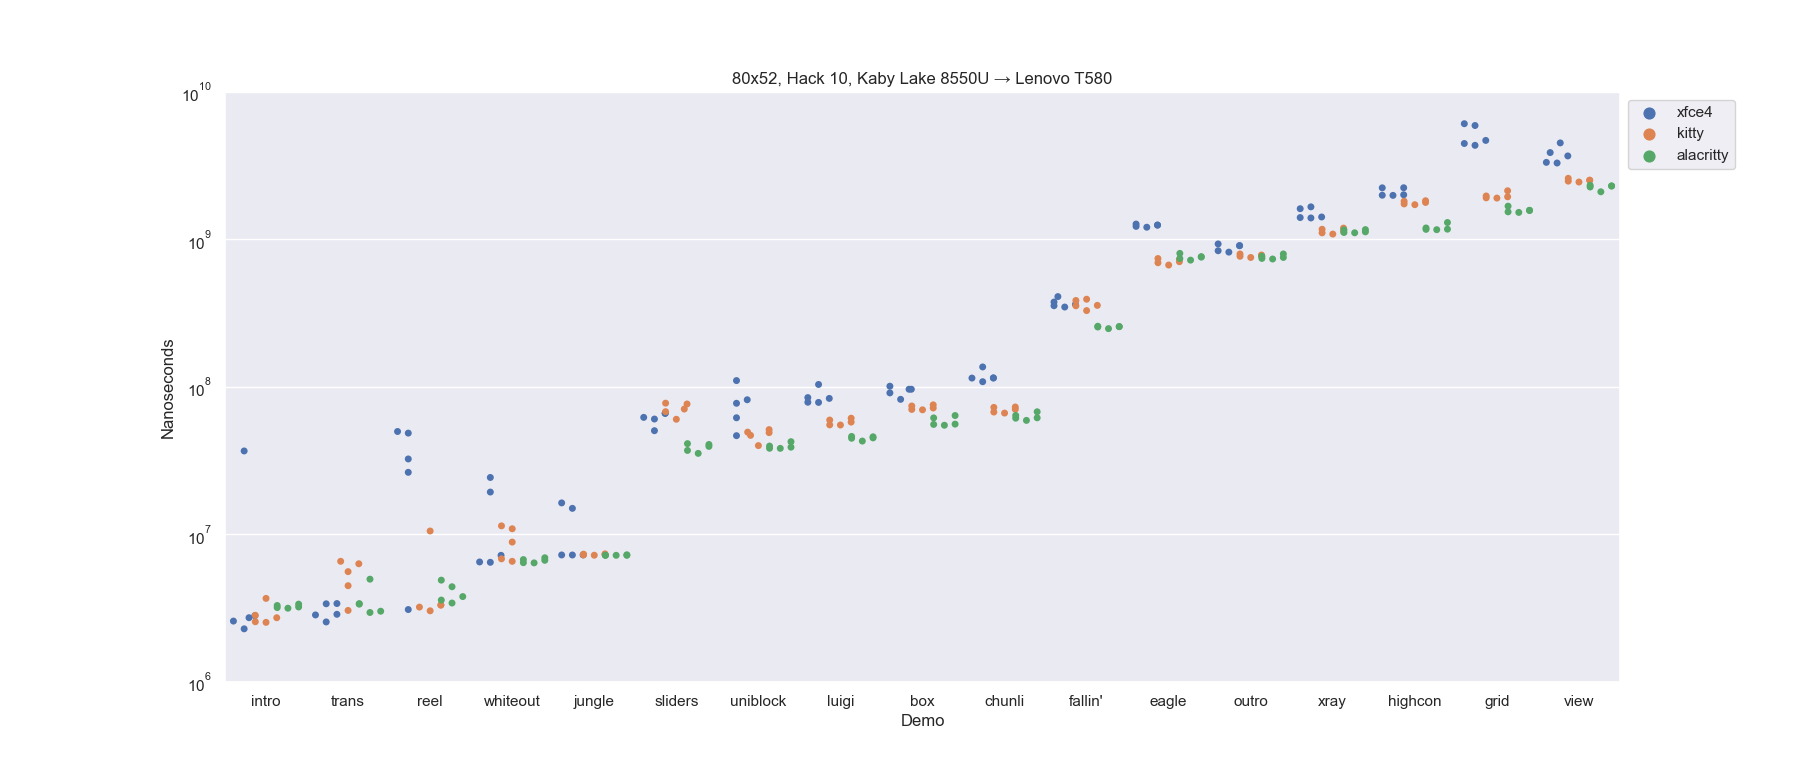
\includegraphics[width=1\textwidth]{media/i915-80x52.png}
\caption[80x52 Intel i7-8550U benchmarks.]{Runtimes on a 80x52 geometry (logarithmic y) atop Linux 5.5.2 + i915, Arch Xorg 1.20.7, no false delay. 5 runs each.}
\label{fig:intel-full}
\end{figure}

\begin{figure}[!htb]
\centering
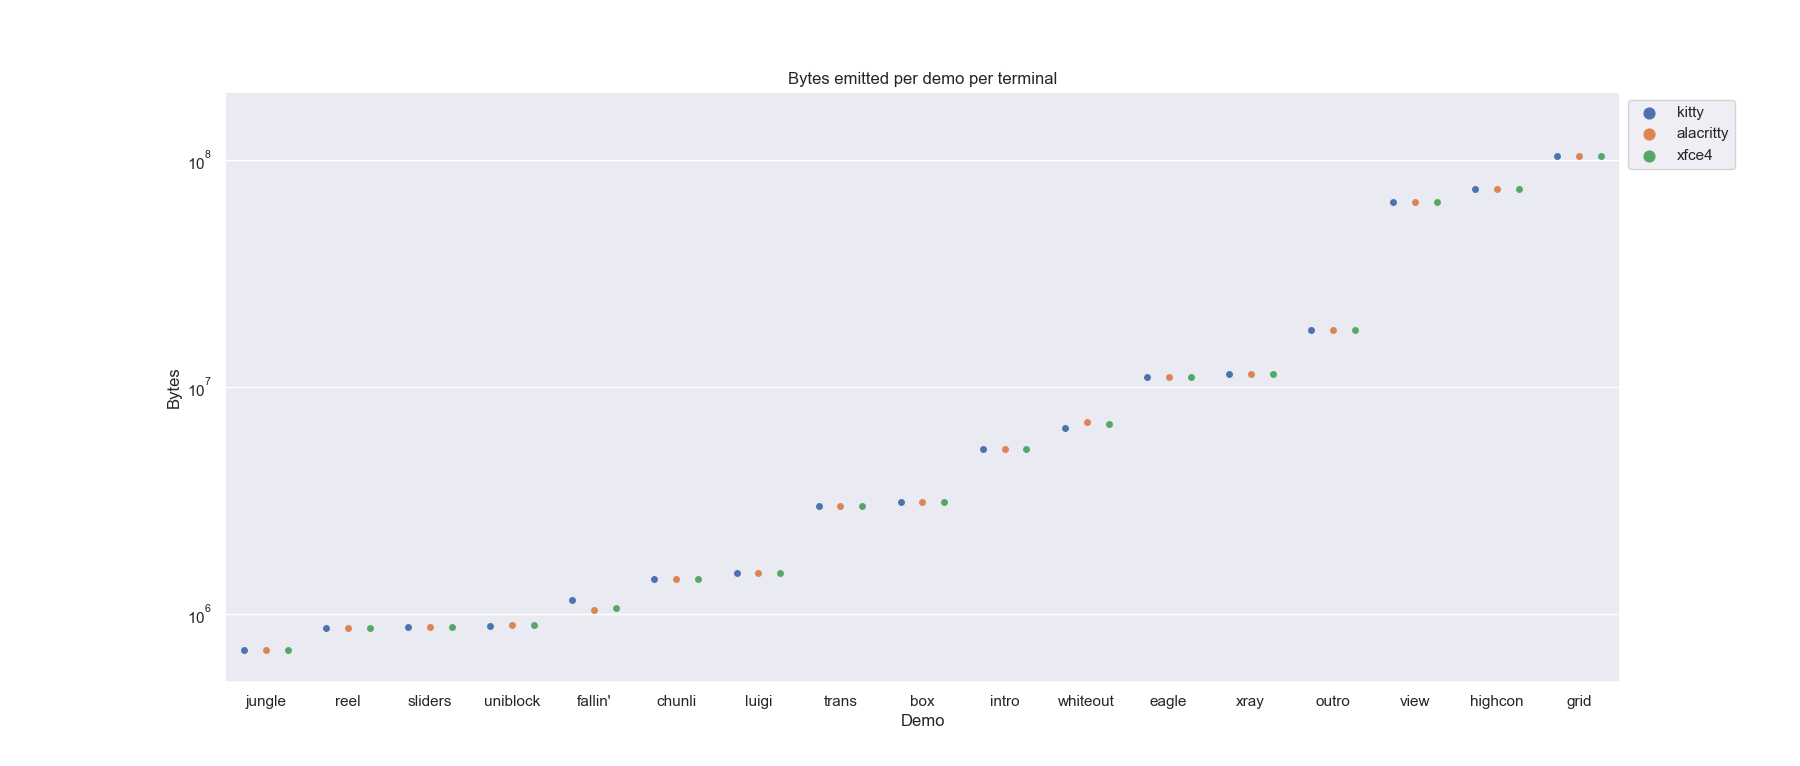
\includegraphics[width=1\textwidth]{media/plotbytes.png}
\caption[Bytes output per demo per term.]{Bytes emitted on a 80x52 geometry (logarithmic y). As expected, the counts are generally equal across terms. If plotted against width, the counts increase linearly.}
\label{fig:nvidia-full}
\end{figure}

\textbf{FIXME FIXME FIXME}
graphs i want:
\begin{denseitemize}
\item{emulator performance as a function of bandwidth--same color everywhere, but turn off elision}
\item{emulator performance as a function of color change--difference with color restored relative to previous}
\item{emulator performance as a function of glyph variation}
\item{some basic perf flame graphs}
\end{denseitemize}
